\subsubsection{monolith::component::layout::BaseLayout}

\label{monolith::component::layout::BaseLayout}
\begin{figure}[ht]
	\centering
	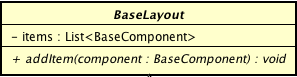
\includegraphics[scale=0.5]{Sezioni/SottosezioniST/img/BaseLayout.png}
	\caption{monolith::component::layout::BaseLayout}
\end{figure}

\begin{itemize}
\item \textbf{Descrizione:} Classe astratta che implementa l'interfaccia BaseComponent e che rappresenta un oggetto layout per la disposizione di componenti nelle bolle di Monolith.
\item \textbf{Utilizzo:} Classe utilizzata ed estesa ogni qualvolta uno sviluppatore intende creare un nuovo layout da inserire in una bolla.
\item \textbf{Attributi:}
\begin{itemize}
\item \textit{private items:List<BaseComponent>}\\
Rappresenta la lista di oggetti BaseComponent contenuti nel layout.
\end{itemize}
\item \textbf{Metodi:}
\begin{itemize}
\item \textit{public addItem(component:BaseComponent):void}\\
Aggiunge un oggetto BaseComponent al layout.
\\ \textbf{Parametri}: \begin{itemize}
\item \textit{component:BaseComponent}\\
Oggetto che rappresenta il BaseComponent da aggiungere al layout.
\end{itemize}
\end{itemize}
\end{itemize}

\subsubsection{monolith::component::layout::vertical::VerticalLayoutView}

\label{monolith::component::layout::vertical::VerticalLayoutView}
\begin{figure}[H]
	\centering
	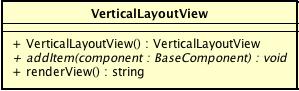
\includegraphics[scale=0.5]{Sezioni/SottosezioniST/img/VerticalLayoutView.png}
	\caption{monolith::component::layout::vertical::VerticalLayoutView}
\end{figure}

\begin{itemize}
\item \textbf{Descrizione:} Classe concreta che estende BaseLayout, destinata alla creazione di layout per la disposizione verticale di BaseComponent.
\item \textbf{Utilizzo:} Classe utilizzata ogni qualvolta uno sviluppatore intende creare un nuovo layout orizzontale da inserire in una bolla.
\item \textbf{Attributi:}
\item \textbf{Metodi:}
\begin{itemize}
\item\textit{public VerticalLayoutView():VerticalLayoutView}\\
Il costruttore per la classe VerticalLayoutView.
\item \textit{public addItem(component:BaseComponent):void}\\
Aggiunge un oggetto BaseComponent al layout verticale.
\\ \textbf{Parametri}: \begin{itemize}
\item \textit{component:BaseComponent}\\
Oggetto che rappresenta il BaseComponent da aggiungere al layout verticale.
\end{itemize}
\item \textit{public renderView():string}\\
Genera il codice HTML, CSS e JavaScript necessario per visualizzare BaseComponent disposti nel layout verticale.
\end{itemize}
\end{itemize}

\subsubsection{monolith::component::layout::horizontal::HorizontalLayoutView}

\label{monolith::component::layout::horizontal::HorizontalLayoutView}
\begin{figure}[H]
	\centering
	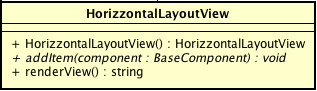
\includegraphics[scale=0.5]{Sezioni/SottosezioniST/img/HorizontalLayoutView.png}
	\caption{monolith::component::layout::horizontal::HorizontalLayoutView}
\end{figure}

\begin{itemize}
\item \textbf{Descrizione:} Classe concreta che estende BaseLayout, destinata alla creazione di layout  per la disposizione orizzontale di BaseComponent.
\item \textbf{Utilizzo:} Classe utilizzata ogni qualvolta uno sviluppatore intende creare un nuovo layout verticale da inserire in una bolla.
\item \textbf{Attributi:}
\item \textbf{Metodi:}
\begin{itemize}
\item\textit{public HorizzontalLayoutView():HorizzontalLayoutView}\\
Il costruttore per la classe HorizzontalLayoutView.
\item \textit{public addItem(component:BaseComponent):void}\\
Aggiunge un oggetto BaseComponent al layout orizzontale.
\\ \textbf{Parametri}: \begin{itemize}
\item \textit{component:BaseComponent}\\
Oggetto che rappresenta il BaseComponent da aggiungere al layout orizzontale.
\end{itemize}
\item \textit{public renderView():string}\\
Genera il codice HTML, CSS e JavaScript necessario per visualizzare BaseComponent disposti nel layout orizzontale.
\end{itemize}
\end{itemize}